\documentclass{article}
\usepackage[utf8]{inputenc}
\usepackage[spanish,es-noshorthands]{babel} % OJO: modificación de la llamada a babel para evitar conflictos con tikz
% https://es.wikibooks.org/wiki/Manual_de_LaTeX/Inclusión_de_gráficos/Gráficos_con_TikZ#Nodos


\usepackage{graphicx} %paquete básico para incluir gráficos
\usepackage{wrapfig} %paquete Wrapfig
\usepackage{float} % paquete para controlar entornos flotantes
\usepackage{pdfpages}% Paquete pdfpages incluye páginas completas de ficheros pdfs
\usepackage{lipsum} % Paquete para introducir texto 
%
\usepackage{tikz} % Paquete TikZ para generar gráficos
\usetikzlibrary{shapes,arrows}


\title{Taller LaTeX Yosigopublicando: Graficos}
\author{ossanche }
\date{March 2021}

\begin{document}

\maketitle

\section{Inclusión de gráficos}

%%%%%%%%%%%%%%%%%%%%%%%%%%%%%%%%%%%%%%%%
\lipsum % incluimos texto
{\bf Final lipsum 1}

\begin{figure}[h]
    \centering
    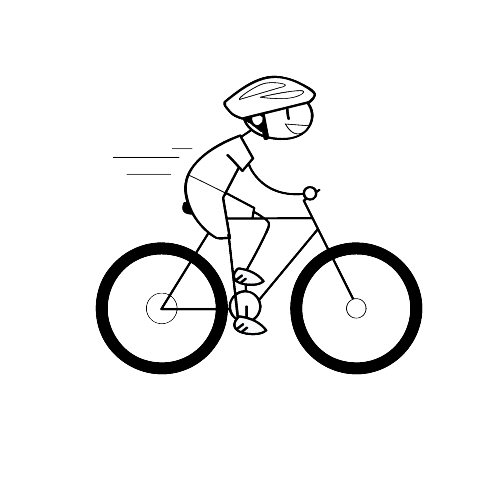
\includegraphics[height=5cm,angle=30]{graficos/ciclista.jpeg}
    \caption{Gráfico simple insertado. \LaTeX lo coloca donde estima oportuno.}
    \label{fig:1}
\end{figure}

Así esta figura puede ser referenciada haciendo una llamada a su etiqueta como se puede apreciar en Figura \ref{fig:1}.

%%%%%%%%%%%%%%%%%%%%%%%%%%%%%%%%%%%%%%%%
\lipsum % incluimos texto
{\bf Final lipsum 2}

\begin{figure}[h]
    \centering
    \frame{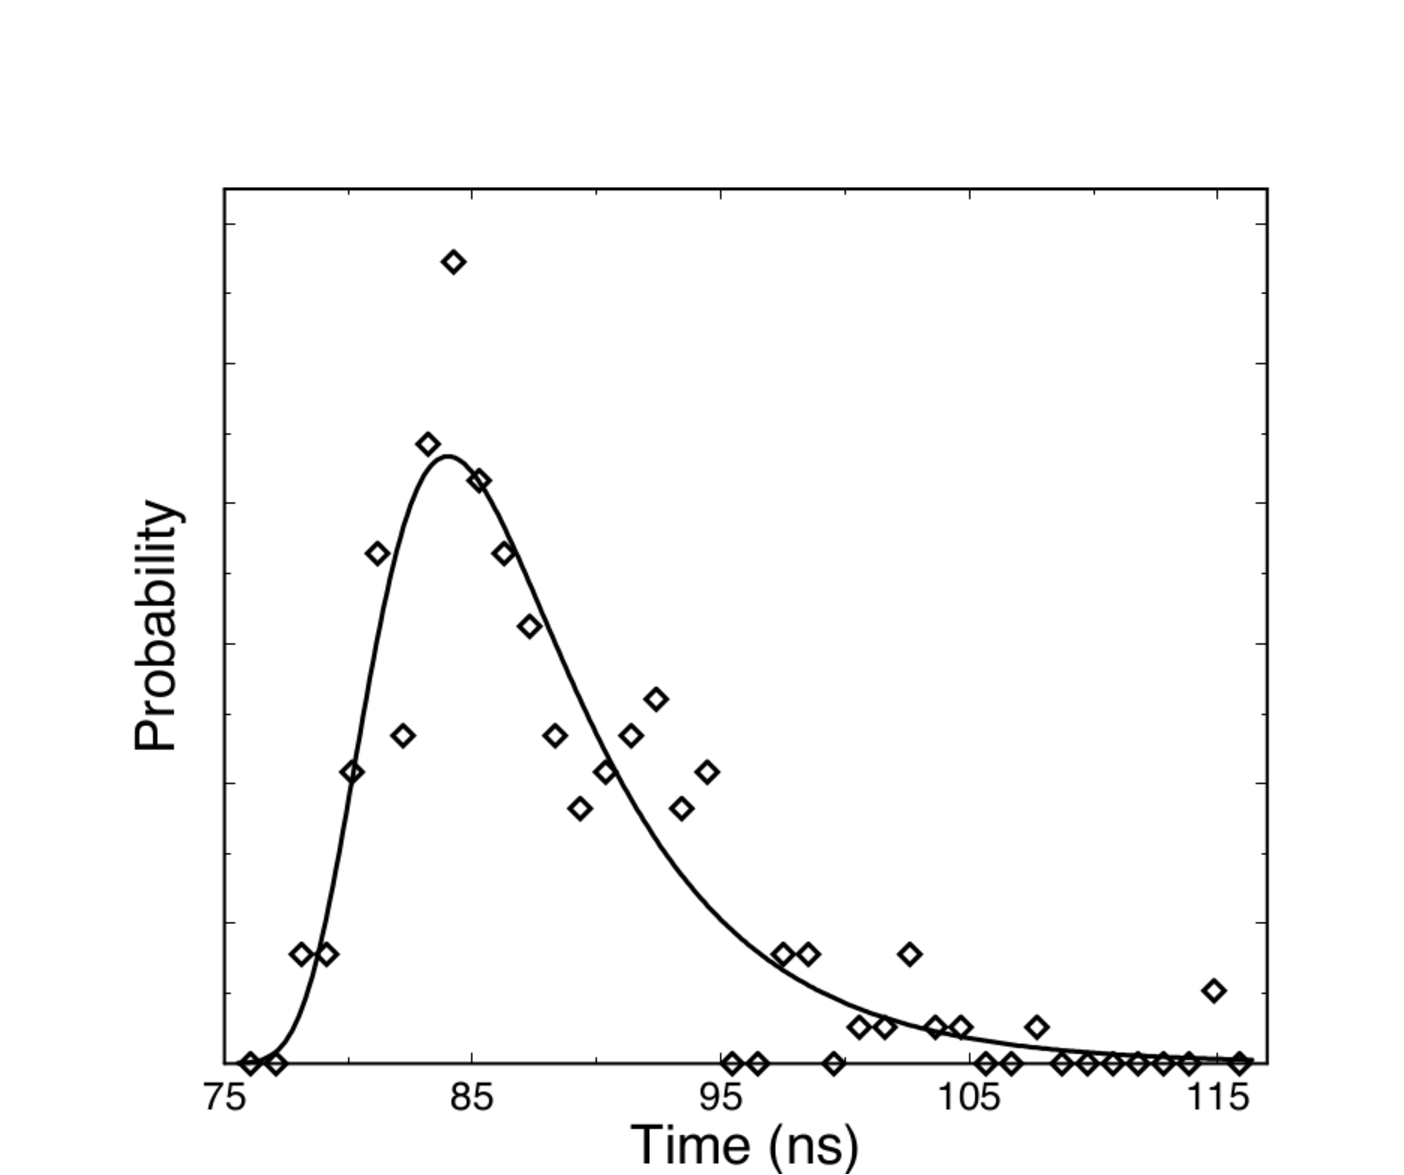
\includegraphics[width=0.45\textwidth]{graficos/fig_9Vis.pdf}}
    \frame{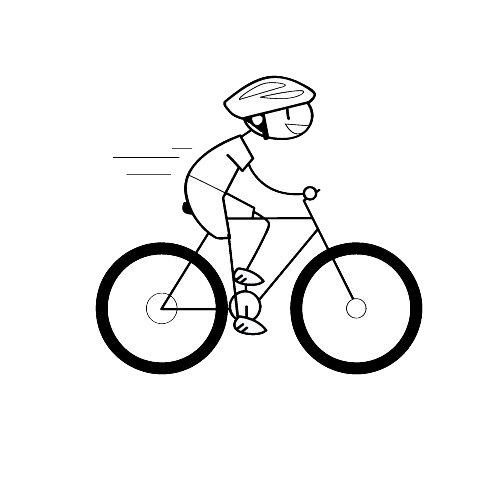
\includegraphics[width=0.45\textwidth]{graficos/ciclista.png}}
    \caption{Dos figuras contiguas. Las incluimos en un marco para poder mejorar su aspecto.}
    \label{fig:2}
\end{figure}


%%%%%%%%%%%%%%%%%%%%%%%%%%%%%%%%%%%%%%%
\lipsum

{\bf Final lipsum 3}

\begin{figure}
    \centering
    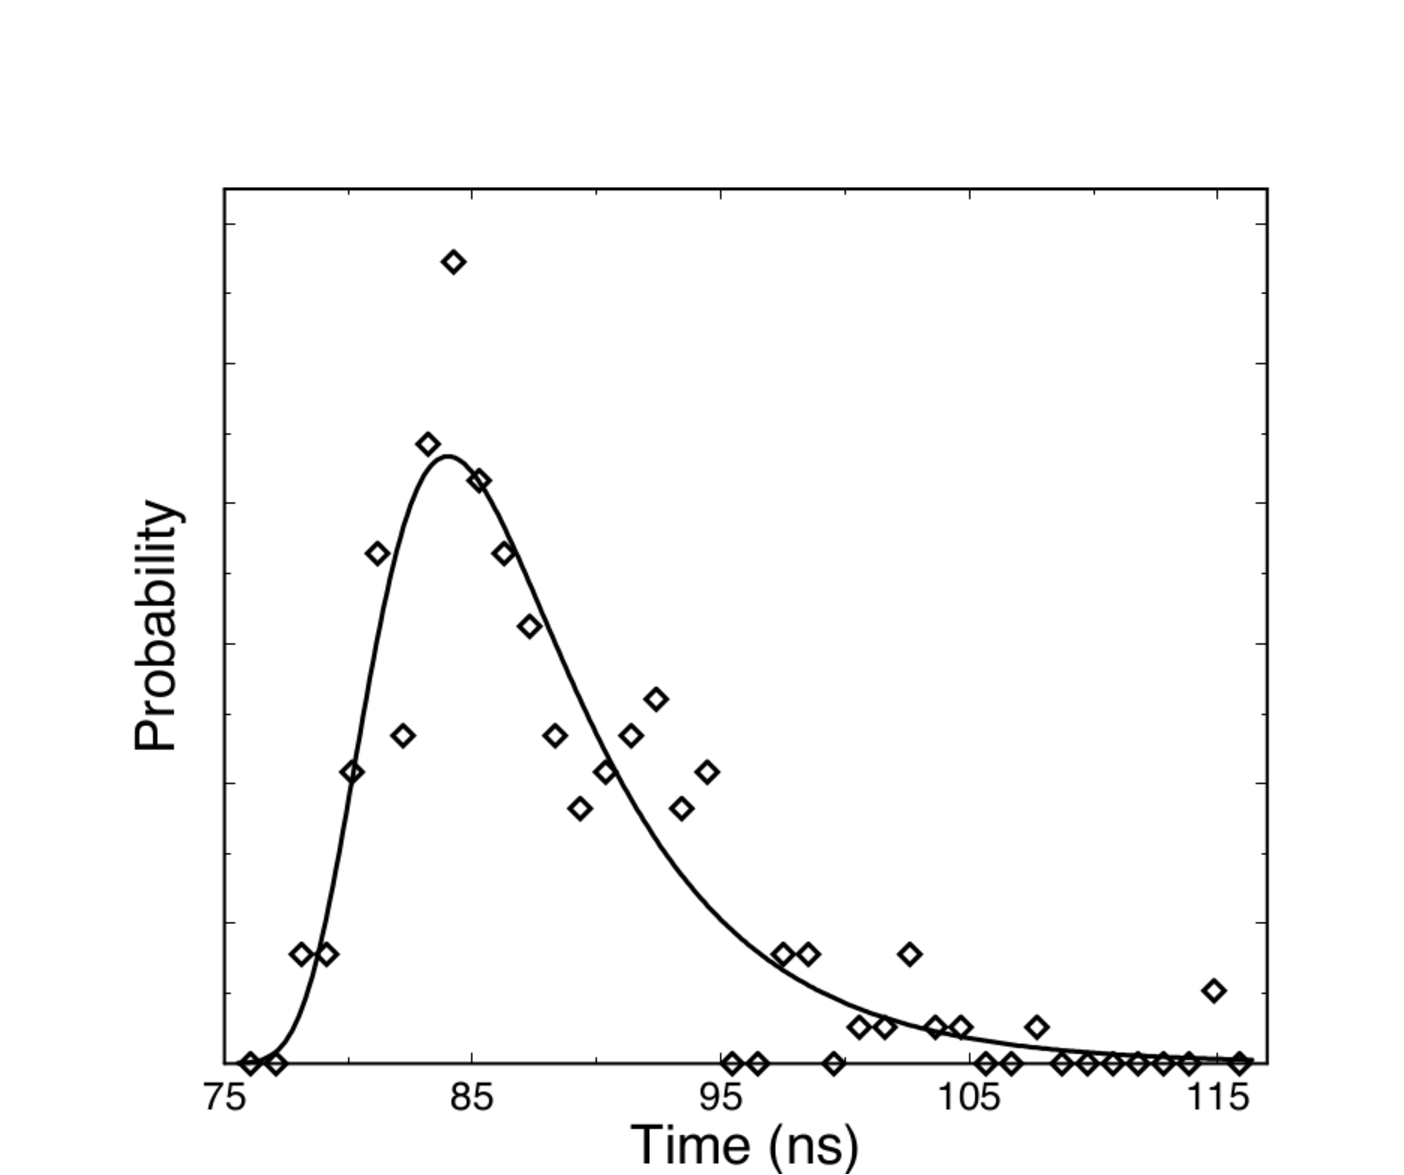
\includegraphics[trim= 0mm 0mm 0mm 30mm,clip,angle=0,width=0.45\textwidth]{graficos/fig_9Vis.pdf}
    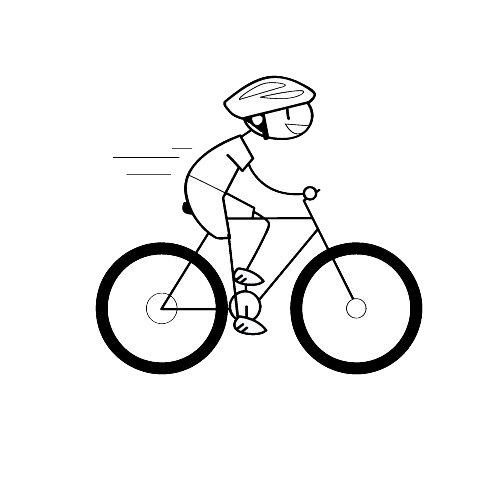
\includegraphics[trim= 0mm 15mm 0mm 5mm,clip,width=0.45\textwidth]{graficos/ciclista.png}
    \caption{Dos imágenes contiguas recortadas para que queden a nivel.}
    \label{fig:3}
\end{figure}

%%%%%%%%%%%%%%%%%%%%%%%%%%%%%%%%%%%%%%%%%%%%
\lipsum

{\bf Final lipsum 4}


\begin{figure}[H] % Requiere paquete float
    \centering
    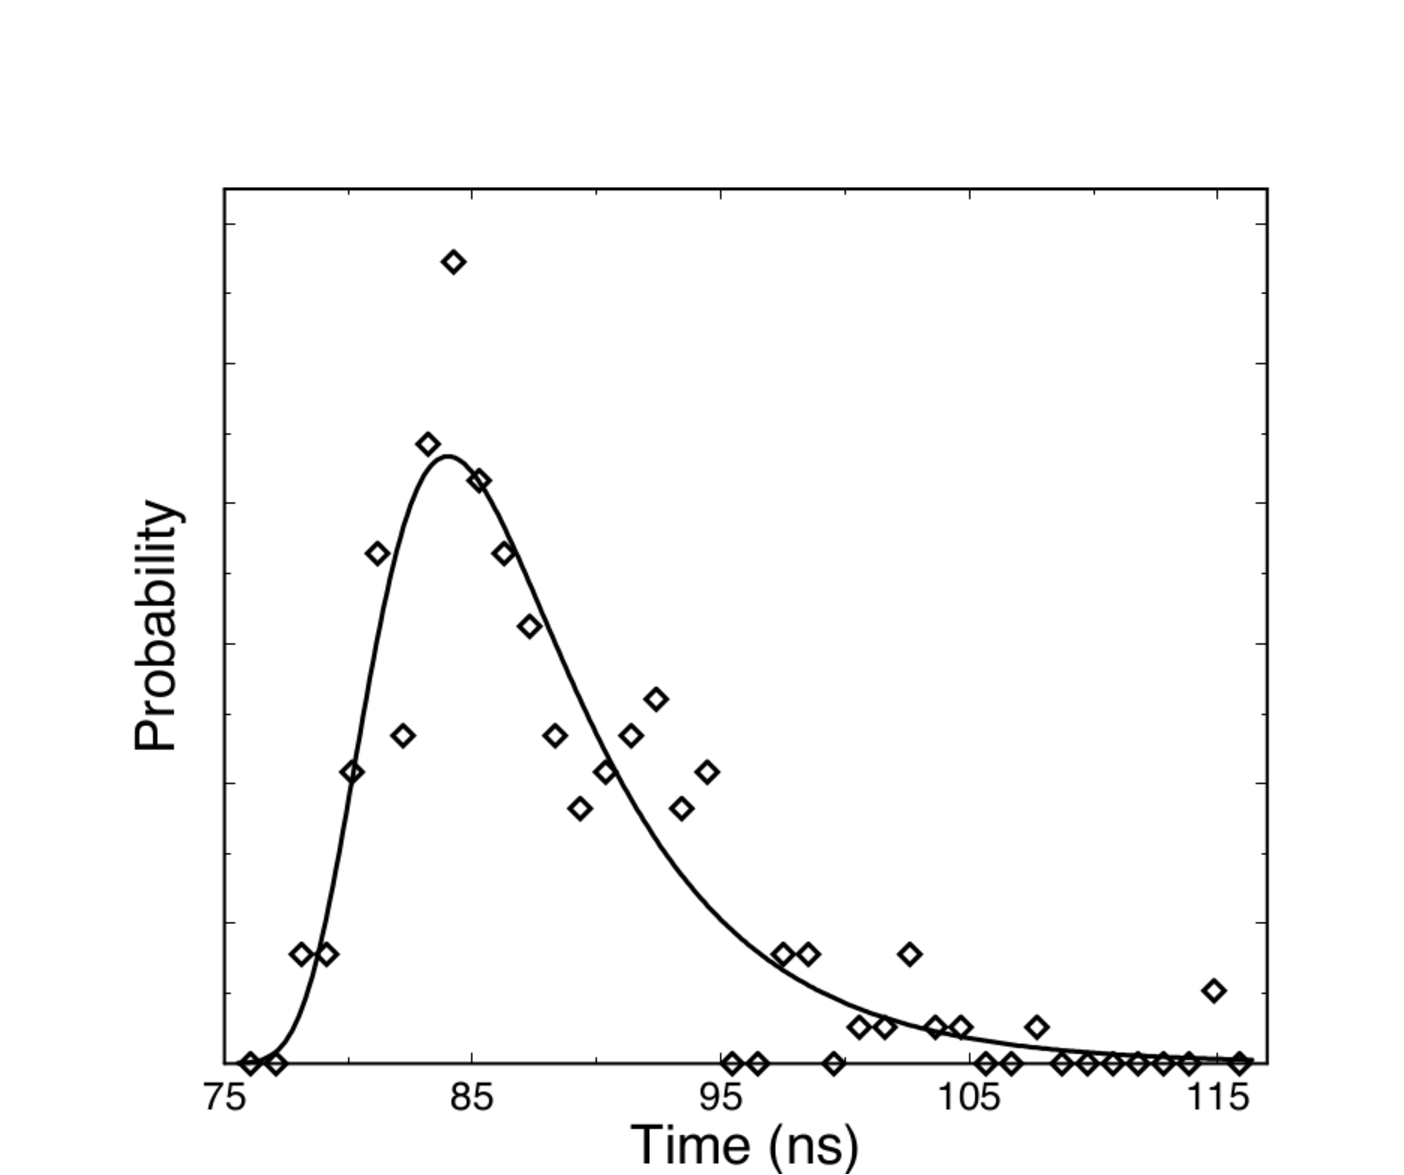
\includegraphics[trim= 0mm 0mm 0mm 30mm,clip,angle=0,width=0.7\textwidth]{graficos/fig_9Vis.pdf}
    \put(-80,150){v=20km/h}
    \put(-100,10){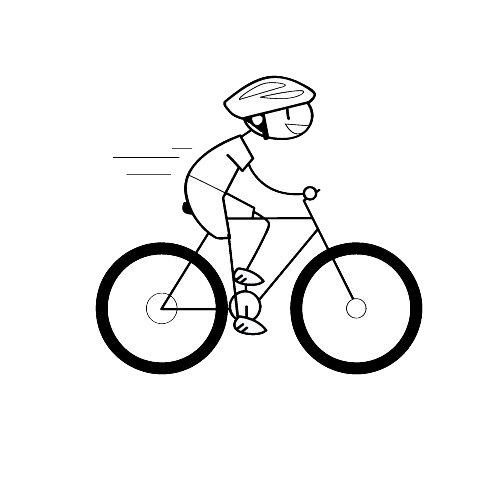
\includegraphics[angle=-7,scale=0.4]{graficos/ciclista.png}}
   % 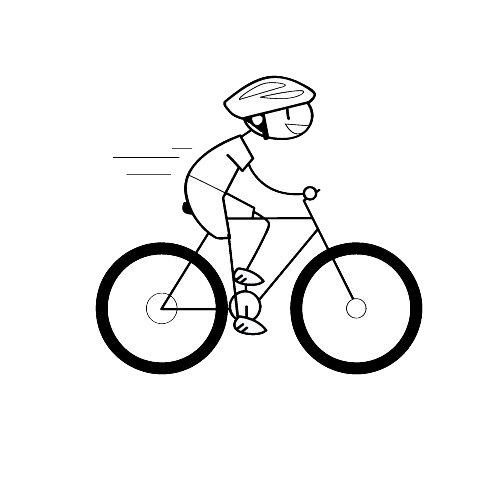
\includegraphics[trim= 0mm 15mm 0mm 5mm,clip,width=0.45\textwidth]{graficos/ciclista.png}
    \caption{Imágen y texto superpuesto. No punto flotante. La responsabilidad de no dejar 
espacios en blanco es nuestra.}
    \label{fig:4}
\end{figure}

\end{document}